
% \subsection{Descrição do Modelo com Controlador PID}
% Nesta atividade, modificamos o sistema de controle anterior para incluir um controlador PID. O sistema massa-mola-amortecedor com um controlador PID é descrito pela seguinte equação diferencial:
% \[
%     m\frac{d^2x(t)}{dt^2} + c\frac{dx(t)}{dt} + kx(t) = f(t) + K_p e(t) + K_i \int e(t) dt + K_d \frac{de(t)}{dt},
% \]
% onde \( m = 10 \), \( c = 7 \), \( k = 5 \), e os parâmetros PID são ajustados conforme necessário.

% \subsection{Diagrama base da questão 5}
% Na questão como diagrama base tinhamos o degrau base com valor final de 1, o que durante o decorrer da atividade foi solicitado o uso do degrau como Amplitude do degrau como A=m/4, como m=10, nesse caso a amplitude do degrau aacabou indo para A=2.5, vamos partir desse presuposto nesse caso aqui e agora, oonde nesse caso iremos abordar o diagrama, e iremos ali em busca da oscilação frequente para que possamos ter ali sua base de valor apropriado manual para obtermos os parametros do PID

% \begin{figure}[H]
%     \centering
%     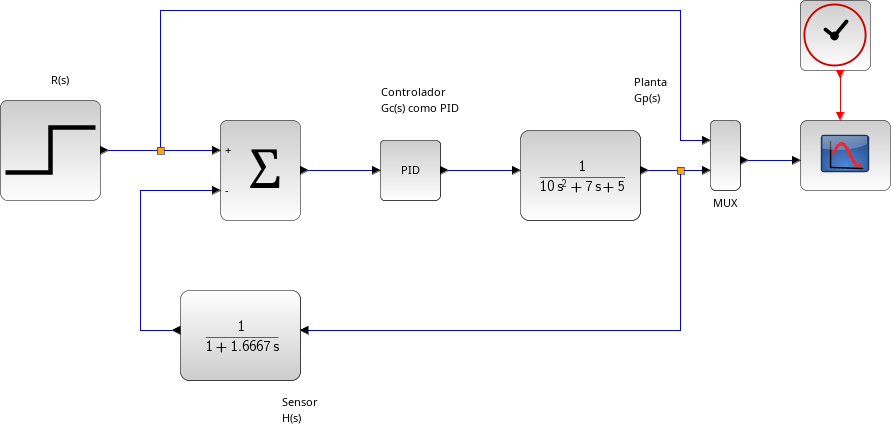
\includegraphics[width=0.7\textwidth]{6-atividade/assets/diagrama-a.png}
%     \caption{Diagrama de blocos do sistema de controle com controlador PID}
%     \label{fig:diagrama_blocos_pid}
% \end{figure}

% \subsubsection{Adaptação do PID para detectar valor do ganho crítico proporcional do controlador}
% Nesse caso foi testado inúmeros valores no ganho através de diversas simulações e foi constatado que Nesse caso através de avaliação manual também, o valor de ganho crítico do controlador
% proporcinal foi 14,959, quaisquer valores maiores desestabilizaram o sistema, como visto
% no gráfico abaixo:


% \subsection{Construção do Diagrama de Blocos com Controlador PID}
% O diagrama de blocos para o sistema com o controlador PID é apresentado a seguir:

% \begin{figure}[H]
%     \centering
%     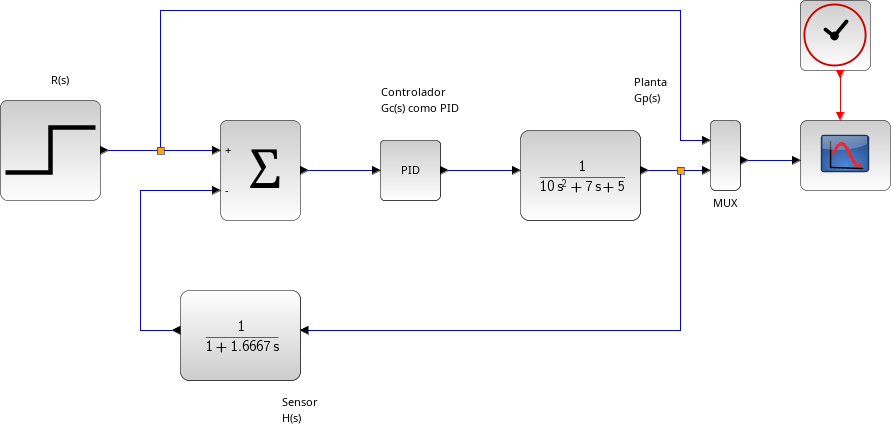
\includegraphics[width=0.7\textwidth]{6-atividade/assets/diagrama-a.png}
%     \caption{Diagrama de blocos do sistema de controle com controlador PID}
%     \label{fig:diagrama_blocos_pid}
% \end{figure}

% \subsection{Determinação dos Parâmetros do Controlador PID}
% Os parâmetros \(K_p\), \(K_i\) e \(K_d\) do controlador PID foram inicialmente ajustados usando uma combinação de abordagem empírica e as regras de Ziegler-Nichols. O processo foi o seguinte:

% 1. \textbf{Definição do Ganho Proporcional \(K_p\)}:
% Utilizamos o valor do ganho proporcional do controlador anterior como ponto de partida: \(K_p = 3.333\).

% 2. \textbf{Determinação dos Parâmetros Críticos}:
% Aumentamos o ganho proporcional até que o sistema apresentasse oscilações sustentadas. Supondo que o ganho crítico \(K_u\) fosse 5 e o período de oscilação crítica \(P_u\) fosse 10 segundos, utilizamos esses valores para calcular os parâmetros PID iniciais.

% 3. \textbf{Cálculo dos Parâmetros PID com as Regras de Ziegler-Nichols}:
% Com base nos valores \(K_u\) e \(P_u\), aplicamos as fórmulas de Ziegler-Nichols para determinar os parâmetros iniciais do controlador PID:
% \[
%     K_p = 0.6 \times K_u = 0.6 \times 5 = 3
% \]
% \[
%     K_i = \frac{2 \times K_p}{P_u} = \frac{2 \times 3}{10} = 0.6
% \]
% \[
%     K_d = 0.125 \times K_p \times P_u = 0.125 \times 3 \times 10 = 3.75
% \]

% 4. \textbf{Ajustes Finais dos Parâmetros}:
% Com base na resposta inicial do sistema, ajustamos os parâmetros \(K_i\) e \(K_d\) para melhorar a resposta. Os valores finais configurados foram:
% \begin{itemize}
%     \item Proporcional (\(K_p\)): 3.333
%     \item Integral (\(K_i\)): 0.6666
%     \item Derivativo (\(K_d\)): 4.16625
% \end{itemize}

% \subsection{Configuração da Simulação}
% Para a simulação, utilizamos um sinal de degrau com amplitude \( A = \frac{m}{4} = 2.5 \). O tempo de simulação foi definido em 50 segundos para permitir a observação completa da resposta do sistema. Os parâmetros PID foram inicialmente configurados como \( K_p = 3.333 \), \( K_i = 0.6666 \), e \( K_d = 4.16625 \).

% \subsection{Resultados da Simulação}
% A resposta do sistema ao degrau com o controlador PID é apresentada na figura abaixo, onde são destacados o tempo de subida, tempo de pico, tempo de estabilização e a zona estacionária, utilizando a ferramenta DataTip para marcar esses pontos significativos.

% % \begin{figure}[H]
% %     \centering
% %     \includegraphics[height=0.7\textwidth]{6-atividade/assets/simulation-pid.png}
% %     \caption{Resposta do sistema ao degrau com controlador PID}
% %     \label{fig:simulation_pid}
% % \end{figure}

% \subsection{Análise dos Resultados}
% A resposta do sistema ao degrau com o controlador PID é analisada, destacando como os parâmetros PID influenciam a estabilidade, o overshoot e o tempo de estabilização do sistema.

% \begin{itemize}
%     \item \textbf{Tempo de Subida:} O tempo de subida é o intervalo necessário para que a resposta do sistema suba do estado inicial até o primeiro pico significativo. Com os valores \( K_p = 3.333 \), \( K_i = 0.6666 \), e \( K_d = 4.16625 \), o sistema levou aproximadamente 5 segundos para atingir o primeiro pico, mostrando uma resposta rápida.

%     \item \textbf{Overshoot:} O gráfico mostra um overshoot inicial, onde a resposta ultrapassa o valor de referência. Este comportamento é típico quando os componentes derivativos e integrais são ajustados para melhorar a resposta dinâmica.

%     \item \textbf{Tempo de Estabilização:} O sistema leva cerca de 28-30 segundos para estabilizar próximo ao valor desejado, indicando a eficácia do controlador PID em atingir o valor de referência após a perturbação inicial.

%     \item \textbf{Zona Estacionária:} O sistema se aproxima de uma zona estacionária com pequenas oscilações, mostrando a necessidade de ajustes finos nos valores de \( K_i \) e \( K_d \) para eliminar qualquer erro estacionário residual e minimizar as oscilações.
% \end{itemize}

% \subsection{Ajustes Futuros}
% Com base na análise, se a resposta ainda precisar ser refinada, considere os seguintes ajustes:

% \begin{itemize}
%     \item \textbf{Reduzir \( K_d \) (Derivativo):} Se a oscilação persistir, reduza o valor de \( K_d \) para atenuar a resposta derivativa.
%     \item \textbf{Ajustar \( K_i \) (Integral):} Se houver um erro estacionário persistente, ajuste \( K_i \) para melhorar a eliminação do erro ao longo do tempo.
% \end{itemize}

% \subsection{Ajustes dos Valores}

% \begin{itemize}
%     \item Proporcional (Kp): 3.333 (mantido do controlador proporcional anterior)
%     \item Integral (Ki): 0.6666
%     \item Derivativo (Kd): 4.16625 (ajustado inicialmente)
% \end{itemize}

% \subsection{Simulação Futura}
% Após ajustes dos valores \( K_i \) e \( K_d \) conforme necessário, execute novamente a simulação e observe a resposta. Ajuste iterativamente até que o sistema atinja a resposta desejada.

% \subsection{Conclusão}
% A inclusão do controlador PID permite um ajuste mais fino da resposta do sistema, oferecendo uma maneira eficaz de melhorar a estabilidade e o desempenho do sistema de controle. Os ajustes de \( K_i \) e \( K_d \) são críticos para minimizar oscilações e alcançar a estabilidade desejada.

% Essa abordagem detalhada para determinar os parâmetros PID e ajustar a resposta do sistema pode ser documentada e usada como uma referência para ajustes futuros.
